In this section we will explain our how our model works and the approached we have used. First we will explain the interactions between the shark and fish before we go in to a more detailed description of how the fish and shark models work.

The fish model used is a combination of previously used models with our own modifications to it. We have created a model of the shark based on multi layer feed forward artificial neural network, trained using a evolutionary  algorithm.

Since we are only interested in modeling the shark when it is hunting we choose to limit our model to only include the phase where the shark has visual contact with the fish shoal. This gives the advantage that we can stop the evaluation in training of sharks that go to far away from the fish. It also let us consider an infinite large sea. The fish are free to move around in the sea without any boundary or periodic boundary. This gives a large performance gain in the training of the neural network.

The movement of the fish and shark is not constrained by any structure or grid. It can however only have discrete coordinates. It is also limited by the model of the animal itself as will be explained below.

The shark and fish shoal positions are updated asynchronously, but the fish in the shoal is updated synchronously. If the shark moves to the position of a fish, the fish is considered eaten by the shark and is as a result removed from the shoal.

Now we will proceed to the more detailed descriptions of the fish and shark model.

\subsection{The fish shoal}

\begin{figure}
\centering
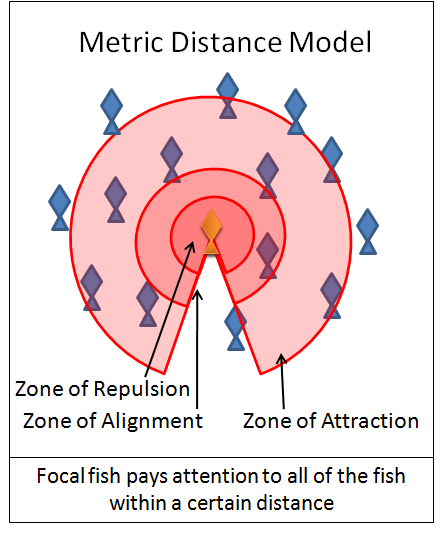
\includegraphics[width=0.45\textwidth]{figs/swarmfig.png}
\caption{\label{fig:swarm} Fish shoal model.}
\end{figure}

The swarming model used is based on the two models found in the references \cite{javafish} and \cite{matlabfish}. It follows the same rules as the basic swarming model, namely repulsion, alignment and attraction. Each of these rules applies at a certain distance range from the fish which can be seen in figure \ref{fig:swarm}. If another fish enters the zone of repulsion they will tend to repel each other and not surprisingly if they are within the attraction distance, they will tend to move towards each other. In the zone of alignment they tend to align themselves so that they will move in the same direction as the other fishes in that zone. Behind the fish there is also a dead zone where no interaction occur (most animals can not see things behind themselves). To further improve the behavior of the swarm, there is also an addition to the algorithm called distance priority \cite{matlabfish}. It makes the fish tend to align itself to the average direction of a set number of its closest neighbors, regardless of which zone they are in.\\
\\
The fishes in the shoal move at a constant drift speed but can accelerate to a max speed to avoid the shark. The way the fishes in this model avoids the shark is quite simple. A scare distance is set for the fishes and should the predator be within this distance, the fish will completely ignore the swarming rules and update the velocity according to
\begin{equation}
\vec{v}_f \rightarrow \vec{v}_f - (\vec{x}_s - \vec{x}_f)a
\end{equation}
where $\vec{v}_f$ is the velocity of the fish, $\vec{x}_s$ the position of the shark, $\vec{x}_f$ the position of the fish and $a$ is a constant called acceleration rate, which decides how fast the fish will be able to reach its max speed (note that the time step is excluded since it will always be set to 1). In other words the fish will just move in opposite direction of where the shark is relative to itself starting at its drift speed and accelerating to its max speed. Having the avoidance rule this way makes for a problem however since this could force a fish to move outside of the attraction zone of the fishes furthest out in the shoal. To solve this it is added that should a fish get too far away from the center of the shoal (average position of all fishes), it will move strictly towards this point if not too close to the shark.

\subsection{The shark}

The model we have created is inspired by nature but not is not an exact description of how sharks behave.

The shark has many senses it can use to detect prey, even on large distances using sight, smell, hearing, electro reception and by detecting vibrations in water, more about this in \cite{shark_vision} and \cite{shark_electric}. Since we have limited ourself to the actual fish catching phase of the hunting we are not interested in the long distance senses.  It is unknown exactly how the all the sharks senses work and it is therefore  difficult to model them, we have chosen an approach that symbolize a combination of the senses in a single sense. The sense model was in our case also limited by the kind of input that were usable with the neural network. The model allows the shark to perceive a fish shoal in front and back of the shark separately as well as the closest fish in the area where the shark is able to catch the fish.

Even though the shark is a very agile predator it can not turn in full speed on the spot, we have therefore constrained the sharks turning angle so that it can only turn $\pi/4$ in each time step. This means that a shark moving at greater speeds will need a larger area for turning.

\subsubsection{Evolution of the artificial neural network of the shark}
gt

The shark is a predator and as such its success in hunting can be measured by the amount of energy spent on the hunt in regards to how much energy it could consume from the prey caught. 
